\documentclass[nobib]{tufte-handout}

%\\geometry{showframe}% for debugging purposes -- displays the margins

\newcommand{\bra}[1]{\left(#1\right)}
\usepackage{amssymb}
\usepackage{hyperref}
\usepackage{pgfplots}
\usepackage{centernot}
\usepackage[activate={true,nocompatibility},final,tracking=true,kerning=true,spacing=true,factor=1100,stretch=10,shrink=10]{microtype}
\usepackage{color}
\usepackage{steinmetz}
% Fixes captions and images being cut off
\usepackage{marginfix}
\usepackage{array}
\usepackage{tikz}
\usepackage{amsmath,amsthm}
\usetikzlibrary{shapes}
\usetikzlibrary{positioning}
\usepackage{listings}
\usepackage{caption}
\DeclareCaptionFont{white}{\color{white}}
\DeclareCaptionFormat{listing}{\colorbox{gray}{\parbox{\textwidth}{#1#2#3}}}
\captionsetup[lstlisting]{format=listing,labelfont=white,textfont=white}

% Set up the images/graphics package
\usepackage{graphicx}
\setkeys{Gin}{width=\linewidth,totalheight=\textheight,keepaspectratio}
\graphicspath{{.}}

\title{Notes for MA 26500 - Linear Algebra I}
\author[Shubham Saluja Kumar Agarwal]{Shubham Saluja Kumar Agarwal}
\date{\today}  % if the \date{} command is left out, the current date will be used

% The following package makes prettier tables.  We're all about the bling!
\usepackage{booktabs}

% The units package provides nice, non-stacked fractions and better spacing
% for units.
\usepackage{units}

% The fancyvrb package lets us customize the formatting of verbatim
% environments.  We use a slightly smaller font.
\usepackage{fancyvrb}
\fvset{fontsize=\normalsize}

% Small sections of multiple columns
\usepackage{multicol}

% For finite state machines 
\usetikzlibrary{automata} % Import library for drawing automata
\usetikzlibrary{positioning} % ...positioning nodes
\usetikzlibrary{arrows} % ...customizing arrows
\tikzset{node distance=2.5cm, % Minimum distance between two nodes. Change if necessary.
    every state/.style={ % Sets the properties for each state
    semithick,
    fill=gray!10},
    initial text={}, % No label on start arrow
    double distance=2pt, % Adjust appearance of accept states
    every edge/.style={ % Sets the properties for each transition
    draw,
    ->,>=stealth', % Makes edges directed with bold arrowheads
    auto,
    semithick}}
\let\epsilon\varepsilon

% These commands are used to pretty-print LaTeX commands
\newcommand{\doccmd}[1]{\texttt{\textbackslash#1}}% command name -- adds backslash automatically
\newcommand{\docopt}[1]{\ensuremath{\langle}\textrm{\textit{#1}}\ensuremath{\rangle}}% optional command argument
\newcommand{\docarg}[1]{\textrm{\textit{#1}}}% (required) command argument
\newenvironment{docspec}{\begin{quote}\noindent}{\end{quote}}% command specification environment
\newcommand{\docenv}[1]{\textsf{#1}}% environment name
\newcommand{\docpkg}[1]{\texttt{#1}}% package name
\newcommand{\doccls}[1]{\texttt{#1}}% document class name
\newcommand{\docclsopt}[1]{\texttt{#1}}% document class option name

% Define a custom command for definitions and biconditional
\newcommand{\defn}[2]{\noindent\textbf{#1}:\ #2}
\let\biconditional\leftrightarrow

\begin{document}

\maketitle

\begin{abstract}
    These are lecture notes for spring 2024 MA 26500 at Purdue as taught by professor Siamak Yassemi. Modify, use, and distribute as you please.
\end{abstract}

\tableofcontents

\section{Course Introduction}
This course serves as an introduction to the fundamental concepts and
applications of linear algebra, a branch of mathematics that explores vector
spaces, linear transformations, and systems of linear equations.

\pagebreak

\section{Systems of Equations in Linear Algebra}
A linear equation is an equation of the form:
\begin{equation*}
    a_1x_1+a_2x_2+...+a_nx_n=b
\end{equation*}
Where $a_1$, $a_2$... and $b$ are given constants.
Note that the exponents of all x terms is 1.
Some examples are:
\begin{equation*}
    2x_1+3x_2=4
\end{equation*}
\begin{equation*}
    5x_1+6x_2=10
\end{equation*}
as opposed to
\begin{equation*}
    2x_1x_2+x_3=9
\end{equation*}
\begin{equation*}
    2x_1+\sqrt{x_2}=8
\end{equation*}
A system of equations is a collection of one or more linear equations involving the same variable set.
An example of this would be:
$$ \begin{cases}
        3x_1 + 5x_2 + x_3 = 3  \\
        7x_1 - 2x_2 + 4x_3 = 4 \\
        -6x_1 + 2x_3 = 2
    \end{cases} $$
where the constant coefficient of $x_2$ in the third equation is 0.\\
A solution is a list of numbers $(s_1, s_2, ..., s_n)$ that makes each equation a true statement when we replace $x_1=s_1$, $x_2=s_2$, ... $x_n=s_n$.
If we have a system of two linear equations, the solution will be the intersection of the two lines that define the equations on the cartesian plane. The system of equations
\begin{align*}
    3x_1-x_2   & = 5 \\
    16x_1-2x_2 & = 6
\end{align*}
is mapped to the following graph:
\begin{center}
    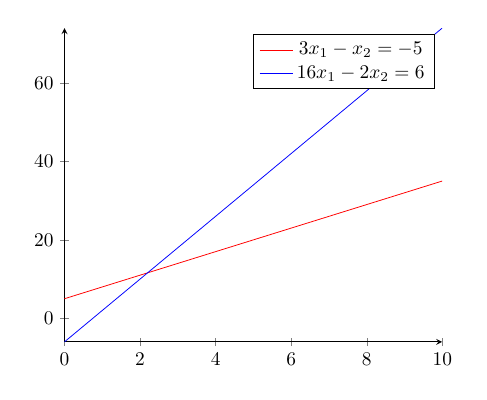
\begin{tikzpicture}[scale = 0.7]
        \begin{axis}[
                axis lines = left,
            ]
            \addplot [
                domain=0:10,
                samples=100,
                color=red,
            ]
            {3*x + 5};
            \addlegendentry{\(3x_1-x_2=-5\)}
            \addplot [
                domain=0:10,
                samples=100,
                color=blue,
            ]
            {8*x - 6};
            \addlegendentry{\(16x_1-2x_2=6\)}

        \end{axis}
    \end{tikzpicture}
\end{center}

There are three kinds of systems:
\begin{enumerate}
    \item One solution
    \item Infinitely many solutions
    \item No solutions
\end{enumerate}
The above example has one solution. This is the intersection of the two lines. This could be further generalized to have far more dimensions as well as far more variables, but such systems are no longer representable in the number of dimensions we can perceive.\\
However, if the lines were parallel, the other two possibilities surge. If the equations are linearly dependent, there would be infinitely many solutions. However, if the value of $b$ were different for the two, while all the variable coefficients were linearly dependent, it would have none.\\
The following is an example of no solution:
\begin{center}
    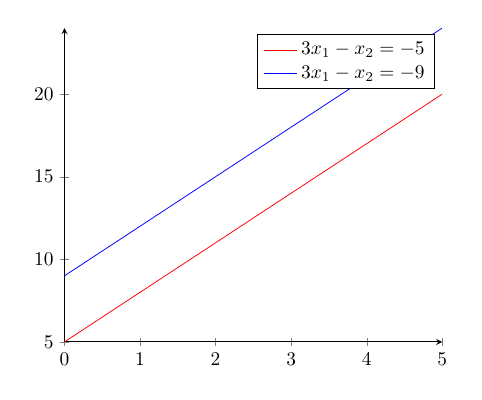
\begin{tikzpicture}[scale = 0.7]
        \begin{axis}[
                axis lines = left,
            ]
            \addplot [
                domain=0:5,
                samples=100,
                color=red,
            ]
            {3*x + 5};
            \addlegendentry{\(3x_1-x_2=-5\)}
            \addplot [
                domain=0:5,
                samples=100,
                color=blue,
            ]
            {3*x + 9};
            \addlegendentry{\(3x_1-x_2=-9\)}
        \end{axis}
    \end{tikzpicture}
\end{center}
While this is infinitely many solutions:
\begin{center}
    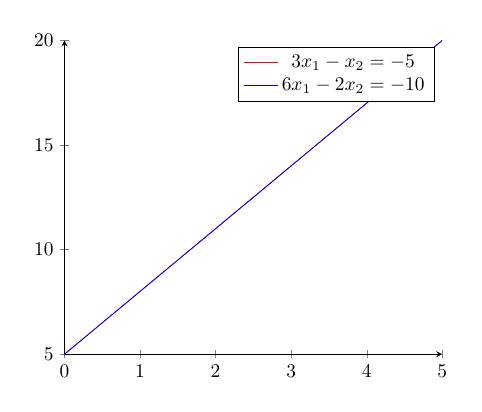
\begin{tikzpicture}[scale = 0.7]
        \begin{axis}[
                axis lines = left,
            ]
            \addplot [
                domain=0:5,
                samples=100,
                color=red,
            ]
            {3*x + 5};
            \addlegendentry{\(3x_1-x_2=-5\)}
            \addplot [
                domain=0:5,
                samples=100,
                color=blue,
            ]
            {3*x + 5};
            \addlegendentry{\(6x_1-2x_2=-10\)}
        \end{axis}
    \end{tikzpicture}
\end{center}
Any system of equations has a matrix notation. For example, the above system can be represented as the following.\\
\begin{equation*}
    \begin{bmatrix}
        3  & -1 & -5 \\
        16 & -2 & 6
    \end{bmatrix}
\end{equation*}
Which has the coefficients of the x values as the first n values, and the value of b as the last one. This is called the augmented matrix of the system of equations. As opposed to:
\begin{equation*}
    \begin{bmatrix}
        3  & -1 \\
        16 & -2
    \end{bmatrix}
\end{equation*}
which is the coefficient matrix.\\
These systems can be solved using the three elementary row operations. This is called row reduction.\\
The three rules are:
\begin{enumerate}
    \item Interchange: Exchange the positions of any two rows
    \item Multiply: Multiply any row by a constant
    \item Addition: Replace the value of a row, with its sum and that of one of the other
          rows multiplied by a scalar.
\end{enumerate}
By using these three rules, one can reduce it to the following form:
\begin{equation*}
    \begin{bmatrix}
        1 & a_2 & a_3 & a_4 \\
        0 & 1   & b_3 & b_4 \\
        0 & 0   & 1   & c_4
    \end{bmatrix}
\end{equation*}
This will result in a trivially solvable unique-solution system of equations. This is also known as a \textbf{consistent} system of equations. We can substitute the value of $x_3$, which is $c_4$, into the equation in the row above, and solve it, as it will now be a single equation with a single variable. This can be done sequentially until all values are found.\\~\\
Note: If the resulting form is instead
\begin{equation*}
    \begin{bmatrix}
        1 & a_2 & a_3 & a_4 \\
        0 & 1   & b_3 & b_4 \\
        0 & 0   & 0   & c_4
    \end{bmatrix}
\end{equation*}
with $c_4 \neq 0$, there would be no solutions, also known as an \textbf{inconsistent} system. On the other hand, if $c_4 = 0$, there will be infinitely many solutions, but it will still be considered a \textbf{consistent} system.
Another point to note is that if the augmented matrices of two systems of equations are equivalent,
that is, if you can transform one matrix into the other through elementary row operations, the systems of equations will have the same solutions.
\pagebreak
\section{Row Reduction and Echelon Forms}
The leading entry of a row refers to the left-most non-zero element in a row.
Thus, the leading entries in the following matrix are:
\begin{equation*}
    \begin{bmatrix}
        \mathbf{1} & 2          & 3          & 4 \\
        0          & \mathbf{6} & 9          & 6 \\
        0          & 0          & \mathbf{8} & 7
    \end{bmatrix}
\end{equation*}
A matrix is in reduced echelon form (REF) if it has the following three properties:
\begin{enumerate}
    \item All non-zero rows are above any rows of all zeros.
    \item Each leading entry in a row is in a column to the right of the leading entry in
          the column above it.
    \item All entries below a leading entry are zeros.\\~\\ If it has the following two
          properties, it will be a row reduced echelon form (RREF):
    \item The leading entry in each non-zero row is 1.
    \item Each leading 1 is the only non-zero element in its column.
\end{enumerate}
Example of echelon form:
\begin{equation*}
    \begin{bmatrix}
        1 & 2 & 5 & 8 \\
        0 & 3 & 9 & 6 \\
        0 & 0 & 9 & 7 \\
        0 & 0 & 0 & 0
    \end{bmatrix}
\end{equation*}
Example of REF:
\begin{equation*}
    \begin{bmatrix}
        1 & 0 & 0 & 8 \\
        0 & 1 & 0 & 6 \\
        0 & 0 & 1 & 7 \\
        0 & 0 & 0 & 0
    \end{bmatrix}
\end{equation*}
\vspace{0.2cm}\\
\textbf{Theorem:} Each matrix is equivalent to one and only one RREF.\\
\quad A pivot position is a location in a matrix that corresponds to a leading 1 in the RREF of a matrix.\\
\quad A pivot column is a column that contains a pivot position.\\~\\
\textit{Tip:} if there is a 1 in the first positions of a row, when the matrix is first "observed", it should be moved to the top of the matrix, as it will most probably make all subsequent computations much easier. \\~\\
\begin{minipage}{\textwidth}
    Row reduction algorithm:
    \begin{enumerate}
        \item Begin with the leftmost non-zero position, and make it the first pivot
              position.
        \item Make all positions under the selected pivot position 0.
        \item Interchange columns to make sure that the rows with the most leading zeros are
              closest to the bottom
        \item Cover the first column and row, and repeat steps 1 to 3 on the resulting
              matrix.
        \item Beginning with the rightmost pivot and working upward and to the left, create
              zeros above each pivot.
    \end{enumerate}
\end{minipage}
\vspace{0.2cm}\\
The solution of the RREF is the solution of the system of equations that has an augmented matrix with the aforementioned RREF.\\
\quad Another thing we can note is that all pivot positions refer to basic variables. If there are any non-pivot columns, the variable referring to these columns will be free.\\
\quad For example a 4x7 matrix is underconstrained and with free variables. \\
\section{Vector Equations}
A matrix with only one column is called a column vector or vector. For example:
\begin{equation*}
    u =
    \begin{bmatrix}
        3 \\
        8 \\
        12
    \end{bmatrix}
    \text{ or } w =
    \begin{bmatrix}
        w_1 \\
        w_2 \\
    \end{bmatrix}
\end{equation*}
Two vectors are equal if and only if their corresponding terms are equal.
There are some basic operations that can be conducted with them.\\
Addition between two vectors of the same size:
\begin{equation*}
    u =
    \begin{bmatrix}
        3 \\
        8 \\
        12
    \end{bmatrix}
    +
    \begin{bmatrix}
        9 \\
        4 \\
        5
    \end{bmatrix}
    =
    \begin{bmatrix}
        3+9 \\
        8+4 \\
        12+5
    \end{bmatrix} =
    \begin{bmatrix}
        12 \\
        12 \\
        17
    \end{bmatrix}
\end{equation*}
Scalar Multiplication:
\begin{equation*}
    u = 3*
    \begin{bmatrix}
        3 \\
        8 \\
        12
    \end{bmatrix}
    =
    \begin{bmatrix}
        3*3 \\
        8*3 \\
        12*3
    \end{bmatrix} =
    \begin{bmatrix}
        9  \\
        24 \\
        36
    \end{bmatrix}
\end{equation*}
Note: these operations both have graphical representations. Addition is addition of two vectors, as is done by the parallelogram method, and scalar multiplication is equivalent to proportionally scaling a vector.\\
A line can be defined as the set of all scalar multiples of a vector.\\
Algebraic properties of a vector in $\mathbb{R}^n$:
\begin{enumerate}
    \item $\mathbf{u}+\mathbf{v} = \mathbf{v}+\mathbf{u}$
    \item $\mathbf{u} + (\mathbf{v}+\mathbf{w}) = (\mathbf{u}+\mathbf{v})+\mathbf{w}$
    \item $\mathbf{u}+\mathbf{0} = \mathbf{u}$
    \item $\mathbf{u}+(-\mathbf{u})=\mathbf{0}$
    \item $c(\mathbf{u}+\mathbf{v}) = c\mathbf{u}+c\mathbf{v}$
    \item $(c+d)\mathbf{u} = c\mathbf{u}+d\mathbf{u}$
    \item  $c(d\mathbf{u}) = cd(\mathbf{u})$
    \item $1\mathbf{u} = \mathbf{u}$
\end{enumerate}
\section{Linear Combinations}
A vector is a linear combination of other vectors if:
\begin{equation*}
    c_1\mathbf{u_1}+c_2\mathbf{u_2}+c_3\mathbf{u_3} \ldots c_n\mathbf{u_n} = \mathbf{v}
\end{equation*}
For any set of vectors, there is an infinite amount of linear combinations, as the values of the constants they are multiplied with are not restrained by anything, and they could be a part of any domain, be it $\mathbb{R}, \mathbb{I}, \text{or } \mathbb{C}$.\\
To find if a vector is a linear combination of other matrices, we can create an augmented matrix with the desired vector as the constant column, and all relevant vectors, as the elements of the coefficient matrix part of the augmented matrix.\\
Should there be a free variable in the resolution of the augmented matrix, there will be infinitely many linear combinations that fulfill the condition we desire.\\
The $span(\mathbf{v_1}, \mathbf{v_2}, \mathbf{v_3}, \ldots, \mathbf{v_n})$ is the set of all linear combinations of these vectors. So, if asked whether a vector is in the span of other vectors, it is equivalent to asking if there exists a linear combination of vectors that results in the desired vector.\\
\section{Matrix Equation \textbf{Ax} = \textbf{b}}
Let $\mathbf{A}$ be an $m\times n$ matrix. The product of $\mathbf{A}$ and $\mathbf{x}$ will be the linear combination of the columns of $\mathbf{A}$ using the entries of $\mathbf{x}$ as weights.
\begin{equation*}
    \mathbf{A}\mathbf{x} =
    \begin{bmatrix}
        \mathbf{a_1} & \mathbf{a_2} & \cdots & \mathbf{a_n}
    \end{bmatrix}
    \begin{bmatrix}
        x_1    \\
        x_2    \\
        \vdots \\
        x_n
    \end{bmatrix} =
    x_1\mathbf{a_1}+x_2\mathbf{a_2}+\cdots+ x_n\mathbf{a_n}
\end{equation*}
Any linear combination can be written in the form $\mathbf{A}\mathbf{x}$, and, if it is a system of linear equations, it can be written as $\mathbf{A}\mathbf{x}=\mathbf{b}$.\\
The matrix equation $\mathbf{A}\mathbf{x}=\mathbf{b}$ has the same solution as $x_1\mathbf{a_1}+x_2\mathbf{a_2}+\cdots+ x_n\mathbf{a_n} = \mathbf{b}$ which in turn has the same solution set as the augmented matrix $\begin{bmatrix}\mathbf{a_1} & \mathbf{a_2} & \cdots & \mathbf{a_n} & \mathbf{b}\end{bmatrix}$.\\
In essence, what we are searching for is the value of $\mathbf{x}$.\\
Existence of solutions:\\
The equation $\mathbf{A}\mathbf{x} =\mathbf{b}$ has a solution if and only if
$\mathbf{b}$ is a linear combination of $\mathbf{A}$.\\ The following
statements are equivalent:
\begin{itemize}
    \item For each $\mathbf{b}$ in $\mathbb{R}^n$ the equation
          $\mathbf{A}\mathbf{x}=\mathbf{b}$ has a solution
    \item The equation $\mathbf{A}\mathbf{x}=\mathbf{b}$ has a solution
    \item Each \textbf{b} in $\mathbb{R}^n$ is a linear combination of the columns of
          $\mathbf{A}$
    \item $\mathbf{A}$ has a pivot position in every row.
\end{itemize}
Row-Vector Rule for Computing \textbf{Ax}:\\
The valid product of two matrices is the sum of the linear combination of each row with their respective terms in the \textbf{x} matrix.\\
\begin{equation*}
    \begin{bmatrix}
        1 & 3 & 4 & 8 \\
        5 & 1 & 4 & 6 \\
        6 & 9 & 1 & 7 \\
        0 & 7 & 4 & 3
    \end{bmatrix}
    \begin{bmatrix}
        x_1 \\
        x_2 \\
        x_3 \\
        x_4
    \end{bmatrix} =
    \begin{bmatrix}
        1x_1+3x_2+3x_3+8x_4 \\
        5x_1+1x_2+4x_3+6x_4 \\
        6x_1+9x_2+1x_3+7x_4 \\
        0x_1+7x_2+4x_3+3x_4
    \end{bmatrix}
\end{equation*}
If \textbf{A} is an $m\times n$ matrix:\
\begin{itemize}
    \item $\mathbf{A(u+v)=Au+Av}$
    \item $\mathbf{A}(\mathbf{u}c) = c(\mathbf{Au})$
\end{itemize}
\section{Solution Sets of Linear Systems}
If a system can be written as $\mathbf{Ax}=0$, it is homogenous. This will
always have the trivial solution of $\mathbf{x}=0$.\\ Thus, there is either a
unique solution or infinitely many solutions. That is, if there is a non-zero
solution, there are infinitely many solutions.\\ This happens because if
$\mathbf{x}$ is a solution, then $c\mathbf{x}$ will also be a solution. The
trivial solution will also need to exist, as anything multiplied by 0 is 0.\\
\quad So, the homogenous equation $\mathbf{Ax}=0$, has a non-trivial solution
if and only if there is a free variable.\\ \quad Suppose $\mathbf{Ax=b}$ is
consistent with solution $\mathbf{p}$, the solution set of the system will be
the set of all the vectors of the form $\mathbf{w=p+v}$ where \textbf{v} is the
solution set of the homogenous equation.\\ 3 planes containing the origin could
have three kinds of intersections:
\begin{enumerate}
    \item Point: origin --- 0 free variables
    \item Line: through origin --- 1 free variable
    \item Plane: same plane through origin --- 2 free variables
\end{enumerate}
This can allow us to express the solution set in terms of vectors scalarly multiplied by the free variables, should there be any.\\
Let us say there are two free variables. All the other variables can be expressed in terms of these free variables.\\
Let us take the following example:
\begin{equation*}
    \begin{bmatrix}
        1 & 2 & 0 & -3 \\
        3 & 6 & 0 & -9 \\
    \end{bmatrix} = 0
\end{equation*}
Has three free variables, and is equivalent to $\begin{bmatrix}1 & 2 & 0 & -3\end{bmatrix} = 0$ with only $x_1$ being non-free.\\
Thus, the solution set can be represented as:
\begin{equation*}
    \mathbf{x}=
    x_2
    \begin{bmatrix}
        -2 \\ 1 \\ 0 \\ 0
    \end{bmatrix} +x_3
    \begin{bmatrix}
        0 \\ 0 \\ 1 \\ 0
    \end{bmatrix} + x_4
    \begin{bmatrix}
        3 \\ 0 \\ 0 \\ 1
    \end{bmatrix}
\end{equation*}
This can be done for any $\mathbb{R}^n$ homogenous matrix.
\begin{enumerate}
    \item Make each free variable 1 for its corresponding $x_n$
    \item Go to each row, and solve the 1 variable equation, with free variable we are
          solving for being 1.
    \item Write the aforementioned solution in the corresponding position of the
          multiplied matrix to $x_n$
\end{enumerate}
\section{Linear Independence}
A set of vectors is linearly independent if the vector equation $\mathbf{Ax=0}$
has only the trivial solution. It is linearly dependent if there exist
solutions distinct to the trivial solution that fulfill the aforementioned
property.\\ The columns of matrix $\mathbf{A}$ are linearly independent if and
only if $\mathbf{Ax=0}$ has only the trivial solution.\\ If every column of A
has a pivot position for $\mathbf{Ax=b}$, there is only one solution, and thus
it is linearly independent.\\~\\ So,
\begin{itemize}
    \item One vector is always linearly independent as long as it is non-zero.
    \item Two vectors are linearly dependent if and only if one vector is a scalar
          multiple of the other.
    \item For three or more vectors, if a vector is a linear combination of the others,
          it is linearly dependent.
\end{itemize}
If a set has more vectors than entries in each vector, then the set is linearly dependent. For example:
\begin{equation*}
    \left\{
    \begin{bmatrix}
        -2 \\ 1 \\
    \end{bmatrix},
    \begin{bmatrix}
        0 \\ 1 \\
    \end{bmatrix},
    \begin{bmatrix}
        3 \\ 0 \\
    \end{bmatrix}
    \right\}
\end{equation*}
\textit{Note: If $\mathbf{A}$ is an $n \times p$ matrix, it has n rows and p unknowns}.\\
If a set contains the $\mathbf{0}$ vector, it is linearly dependent.\\
\section{Introduction to Linear Transformations}
A transformation or function $T$ from $\mathbb{R}^n$ to $\mathbb{R}^m$ is a
rule that takes each vector in $\mathbb{R}^n$ and assigns to it a vector in
$\mathbb{R}^m$.\\ The set $\mathbb{R}^n$ is called the domain, and the set
$\mathbb{R}^m$ is called the codomain of $T$.\\ The notation is:
\begin{equation*}
    T: \mathbb{R}^n \rightarrow \mathbb{R}^m
\end{equation*}
so $\mathbf{x}\in\mathbb{R}^n$ and $T(\mathbf{x})\in\mathbb{R}^m$.\\
A Matrix Transformation consists of a matrix $m\times n$ can define a transformation from $\mathbb{R}^n$ to $\mathbb{R}^m$.
That is:
\begin{equation*}
    \mathbf{x \mapsto A_{n\rightarrow m}x}
\end{equation*}
or
\begin{equation*}
    T(\mathbf{x})=\mathbf{Ax}
\end{equation*}
In essence, a matrix transformation is the multiplication of the matrix \textbf{x} with a matrix \textbf{A} that results in the final transformed matrix that we desire.\\
So, when asked about the existence of $T(\mathbf{x})=\mathbf{b}$, all that is necessary is the creation and resolution of the augmented matrix of \textbf{A} and \textbf{b}.\\
This allows for a multitude of geometric transformations such as:
\begin{center}
    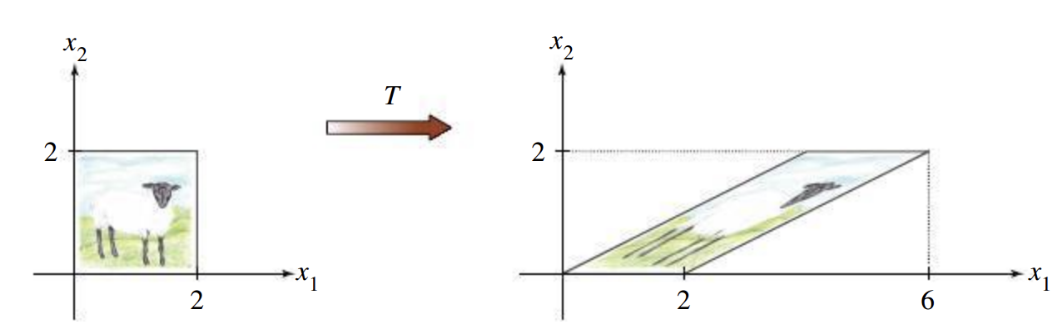
\includegraphics[width = 200px]{images/transformation_use.png}
\end{center}
A linear transformation has the following properties:
\begin{itemize}
    \item $T(\mathbf{u+v})=T(\mathbf{u})+T(\mathbf{v})$
    \item $T(c\mathbf{u})=cT(\mathbf{u})$
    \item $T(\mathbf{0})=\mathbf{0}$ --- which is quite useful for an initial verification of linear transformations
    \item $T(c\mathbf{u}+d\mathbf{v})= cT(\mathbf{u})+dT(\mathbf{v})$
\end{itemize}
\textit{Note: all matrix transformations are linear transformations, but not all linear transformations are matrix transformations.}\\
If a matrix is in the range of $T$, it is a linear transformation of the columns of the matrix \textbf{A} that defines $T(x)$.\\
Let $T$ be a linear transformation. There exists a matrix such that $T(\mathbf{x})=\mathbf{Ax}$. So, we will now work on finding \textbf{A}.\\
We know that:
\begin{equation*}
    T
    \begin{bmatrix}
        x_1 \\ x_2 \\
    \end{bmatrix} = T\left(x_1
    \begin{bmatrix}
        1 \\ 0 \\
    \end{bmatrix}+x_2
    \begin{bmatrix}
        0 \\ 1 \\
    \end{bmatrix}\right)
\end{equation*}
For any linear transformation there exists a unique matrix \textbf{A}, called the standard matrix of $T$, that, in most cases, can be found using the above property.\\
One just needs to find the values of the transformation of all the vectors of the form:
\begin{equation*}
    \begin{bmatrix}
        0 \\ 0 \\ \vdots \\ 1 \\ \vdots \\0\\0
    \end{bmatrix}
\end{equation*}
and each transformation of each vector will be it's respective column of the matrix \textbf{A}.\\
A transformation is one-to-one if for each point in $\mathbb{R}^m$, that is, the range, every point has at most one vector in $\mathbb{R}^n$ that transforms into it.\\
A transformation is onto if for each point in $\mathbb{R}^n$, that is, the domain, every point has a transformation.\\
\begin{itemize}
    \item A linear transformation $T$ is one-to-one if and only if $T(x)=0$ has just the
          trivial solution.
    \item $T$ is one-to-one $\iff$ the columns are linearly independent.
    \item $T$ maps $\mathbb{R}^n$ onto $\mathbb{R}^m$ $\iff$ the columns of \textbf{A} span $\mathbb{R}^m$.
    \item $T$ is onto $\iff$ there is a pivot position in every row.
    \item If $n>m$, the transformation cannot be one-to-one.
    \item If $m>n$, the transformation cannot be onto.
    \item If $m=n$, $T$ is onto $\iff$ $T$ is one-to-one.
\end{itemize}
\section{Matrix Operations}
\begin{itemize}
    \item Sum:\\
          \begin{equation*}
              u =
              \begin{bmatrix}
                  3 \\
                  8 \\
                  12
              \end{bmatrix}
              +
              \begin{bmatrix}
                  9 \\
                  4 \\
                  5
              \end{bmatrix}
              =
              \begin{bmatrix}
                  3+9 \\
                  8+4 \\
                  12+5
              \end{bmatrix} =
              \begin{bmatrix}
                  12 \\
                  12 \\
                  17
              \end{bmatrix}
          \end{equation*}
          Requires the matrices to be the same size.\\~\\
    \item Scalar multiplication:
          \begin{equation*}
              u = 3*
              \begin{bmatrix}
                  3 \\
                  8 \\
                  12
              \end{bmatrix}
              =
              \begin{bmatrix}
                  3*3 \\
                  8*3 \\
                  12*3
              \end{bmatrix} =
              \begin{bmatrix}
                  9  \\
                  24 \\
                  36
              \end{bmatrix}
          \end{equation*}
          If \textbf{A,B,C} are matrices of the same size:\
          \begin{itemize}
              \item $\mathbf{A+B=B+A}$
              \item $\mathbf{(A+B)+=A+(B+C)}$
              \item $\mathbf{A+0=A}$
              \item $r\mathbf{(A+B)=}r\mathbf{A}+r\mathbf{B}$
              \item $(r+s)\mathbf{A=}r\mathbf{A}+s\mathbf{A}$
              \item $r(s\mathbf{A}) = s(r\mathbf{A})$
          \end{itemize}
    \item Matrix Multiplication:\\ Let \textbf{A} be an $m\times n$ matrix and \textbf{B}
          be an $n\times p$ matrix, and \textbf{B} has the columns
          $\mathbf{b_1,b_2,\ldots,b_n}$. \textbf{AB} is defined as the matrix with
          columns $\mathbf{Ab_1,Ab_2,\ldots,Ab_n}$.\\ \textit{Note: the number of columns
              of \textbf{A}, is the same as the number of rows of \textbf{B}}.
          \begin{equation*}
              \begin{bmatrix}
                  3  & 4 \\
                  8  & 5 \\
                  12 & 1
              \end{bmatrix}
              \begin{bmatrix}
                  2 & 1 \\
                  1 & 3 \\
              \end{bmatrix}
              =
              \begin{bmatrix}
                  3(2)+4(1)  & 3(1)+4(3)  \\
                  8(2)+5(1)  & 8(1)+5(3)  \\
                  12(2)+1(1) & 12(1)+1(3)
              \end{bmatrix} =
              \begin{bmatrix}
                  10 & 15 \\
                  21 & 23 \\
                  25 & 15
              \end{bmatrix}
          \end{equation*}
          Let $\mathbf{A}_{ij}$ be the entry in row $i$ and column $j$ of matrix \textbf{A}.
          \begin{equation*}
              (\mathbf{AB})_{ij} = \mathbf{A}_{i1}\mathbf{B}_{1j}+\mathbf{A}_{i2}\mathbf{B}_{2j}+\mathbf{A}_{i3}\mathbf{B}_{3j}+\cdots+\mathbf{A}_{in}\mathbf{B}_{nj}
          \end{equation*}
          Matrix multiplication has the following properties:
          \begin{itemize}
              \item $\mathbf{A(BC)=(AB)C}$
              \item $\mathbf{A(B+C)=AB+AC}$
              \item $\mathbf{(B+C)A=BA+CA}$
              \item $r\mathbf{(AB)=(\textit{r}A)B = A(\textit{r}B)}$
              \item $\mathbf{I_mA=A = AI_m}$
          \end{itemize}
          with $\mathbf{I_m}$ being the identity matrix.\\
          \textit{Note: $\mathbf{AB \neq BA}$} unless $\mathbf{B=I_n}\lor \mathbf{B=0}$\\
          \textit{Note: $\mathbf{AB=0} \centernot\implies \mathbf{A=0}\lor \mathbf{B=0} $}\\
          Powers of a matrix:\\
          If \textbf{A} is an $n\times n$ matrix, then $\mathbf{A}^k$ is the matrix that results from:
          \begin{equation*}
              \mathbf{A}^k = \underbrace{\mathbf{A} \times \mathbf{A} \times \cdots \times \mathbf{A}}_{\text{k times}}
          \end{equation*}
    \item Transpose of a Matrix:\\ Given an $m\times n$ matrix, the transpose of this
          matrix is the $n\times m$ matrix, denoted by $\mathbf{A}^T$, whose columns are
          formed by the corresponding rows of \textbf{A}.
          \begin{equation*}
              \begin{bmatrix}
                  a & b \\
                  c & d \\
                  e & f
              \end{bmatrix}^T
              =
              \begin{bmatrix}
                  a & c & e \\
                  b & d & f \\
              \end{bmatrix}
          \end{equation*}
          It has the following properties:
          \begin{itemize}
              \item $(\mathbf{A}^{T})^T = \mathbf{A}$
              \item $\mathbf{A+B}^{T} = \mathbf{A}^T+\mathbf{B}^T$
              \item $(r\mathbf{A})^{T} = r\mathbf{A}^T$
              \item $(\mathbf{AB})^{T} = \mathbf{A}^T\mathbf{B}^T$
          \end{itemize}
\end{itemize}
Let \textbf{A} be an $n\times n$ matrix. This means \textbf{A} is a square matrix.\\
If this \textbf{A} is of the form:
\begin{equation*}
    \begin{bmatrix}
        a & b & c \\
        0 & d & e \\
        0 & 0 & f
    \end{bmatrix}
\end{equation*}
it is an upper triangular matrix.\\
If this \textbf{A} is of the form:
\begin{equation*}
    \begin{bmatrix}
        a & 0 & 0 \\
        b & c & 0 \\
        d & e & f
    \end{bmatrix}
\end{equation*}
it is a lower triangular matrix.\\
If this \textbf{A} is of the form:
\begin{equation*}
    \begin{bmatrix}
        a & 0 & 0 \\
        0 & b & 0 \\
        0 & 0 & c
    \end{bmatrix}
\end{equation*}
it is a diagonal matrix.\\
If this \textbf{A} is of the form:
\begin{equation*}
    \begin{bmatrix}
        0 & 0 & 0 \\
        0 & 0 & 0 \\
        0 & 0 & 0
    \end{bmatrix}
\end{equation*}
it is a zero matrix.\\
\section{Inverse of a Matrix}
An $n\times n$ matrix \textbf{A} is said to be invertible, if there is an
$n\times n$ matrix \textbf{C} such that $\mathbf{CA=AC=I_n}$. If it is not
invertible, it is singular. Thus, if it is invertible, it is also
non-singular.\\ The inverse of $\mathbf{A}$ is denoted by $\mathbf{A^{-1}}$.\\
Let $\mathbf{A} = \begin{bmatrix}
        a & b \\
        c & d
    \end{bmatrix}$. If $ab-cd \neq 0$, \textbf{A} is invertible and $\mathbf{A^{-1}} = \frac{1}{ad-bc}\begin{bmatrix}
    d  & -b \\
    -c & a
\end{bmatrix}$.\\
\begin{center}
    \textit{Note: $ad-bc$ is called the determinant of the matrix.}\\    
\end{center}
If \textbf{A} is invertible, for any \textbf{b} in $\mathbb{R}^n$, the equation $\mathbf{Ax=b}$ has the unique solution $\mathbf{x=A^{-1}b}$.\\
This has a few additional properties:
\begin{itemize}
    \item If \textbf{A} is invertible, then $\mathbf{A^{-1}}$ is also invertible, and $\mathbf{A = (A^{-1})^{-1}}$
    \item If \textbf{A} and \textbf{B} are both invertible, than \textbf{AB} is invertible and $\mathbf{(AB)^{-1} = A^{-1}B^{-1}}$.
    \item If \textbf{A} is invertible, then $\mathbf{A^T}$ is invertible and $\mathbf{(A^T)^{-1} = (A^{-1})^T}$.
\end{itemize}
An elementary matrix is defined as a matrix that can be obtained from performing a single elementary operation on the identity matrix.\\
If an elementary operation is performed on an $n\times n$ matrix \textbf{A}, the resulting matrix can be represented by \textbf{EA}, where \textbf{E} is the result of the same operation applied to the identity matrix.\\
This will allow us to define any matrix that results from elementary operations of another as a multiplication of elementary matrices with the original matrix.\\
A matrix \textbf{A} is invertible $\iff$ \textbf{A} is row equivalent to $\mathbf{I_n}$.\\
The algorithm to find $\mathbf{A^{-1}}$ for any matrix is the following:
\begin{enumerate}
    \item Write down the matrix $\mathbf{[A|I_n]}$.
    \item Row reduce \textbf{A} until it is equal to $\mathbf{I_n}$.
    \item Perform the same operations to $\mathbf{I_n}$.
    \item The result of what was originally $\mathbf{I_n}$ will be $\mathbf{A^{-1}}$.
\end{enumerate}
If we have a square matrix $\mathbf{A}$ of size $n\times n$:
\begin{itemize}
    \item $\mathbf{A}$ is invertible
    \item $\mathbf{A}$ is row equivalent to $\mathbf{I_n}$
    \item $\mathbf{A}$ has $n$ pivot positions
    \item $\mathbf{Ax = 0}$ has only the trivial solution
    \item Columns of \textbf{A} are linearly independent
    \item The linear transformation $\mathbf{x\mapsto Ax}$ is one-to-one
    \item The equation $\mathbf{Ax=b}$ has at least one solution for each \textbf{b} in $\mathbb{R}^n$
    \item The columns of \textbf{A} span $\mathbb{R}^n$
    \item The linear transformation $\mathbf{x\mapsto Ax}$ maps $\mathbb{R}^n$ to $\mathbb{R}^n$
    \item There is an $n \times n$ matrix \textbf{C} such that $\mathbf{CA = I}$
    \item There is an $n \times n$ matrix \textbf{D} such that $\mathbf{AD = I}$
    \item $\mathbf{A^T}$ is an invertible matrix
\end{itemize}
\end{document}